\documentclass[conference]{IEEEtran}

\usepackage{amsmath}
\usepackage{amssymb}
\usepackage{graphicx}
\usepackage{booktabs}
\usepackage{hyperref}
\usepackage{url}
\usepackage{balance}

\graphicspath{{../results/}}

\begin{document}

\title{A Markov-Chain Approach to Citation-Based Paper Recommendation}

\author{%
\IEEEauthorblockN{Hayden Leung (cl4627), Rea Lila (rl3512), Mireille Donoso-Kugler (md4418)}
\IEEEauthorblockA{Columbia University}
}

\maketitle

\begin{abstract}
We model academic paper recommendation as Personalized
PageRank on a citation network built around a single seed
paper, scraped two hops outward via breadth-first search. The
ranking we want comes out as the invariant distribution of a
Markov chain whose walker, at each step, either follows a
citation or teleports back to the seed; dangling nodes
(papers with no recorded outgoing citations) are also
redirected to the seed. To compute it, we solve a sparse linear system derived from
this chain. We then test two predictions about the method's
behavior. First, power iteration converges geometrically
at a rate set by the damping factor times the magnitude of the
second-largest eigenvalue of the transition matrix, with the
observed contraction matching the spectral prediction within
one percent. Second, the resulting ranking barely moves as we vary the
damping factor across the range we tested: pairwise Pearson
correlation between score vectors stays above 0.994 for every
pair of damping values. On the seed
\emph{Attention Is All You Need}, the method produces a
reading list that overlaps with raw citation count on 18 of 20
papers, with the remainder reflecting structural relevance
beyond popularity.
\end{abstract}

\section{Introduction}
\label{sec:intro}

Literature review for a new topic has a cold-start problem. A
researcher comes across one interesting paper and wants to
understand its intellectual neighborhood: the prior work it
builds on, the follow-ups it has sparked, and the papers it
should be read alongside. Keyword search is a blunt instrument
for this because the right neighbors often share no surface
terms. Citation count is a more structural alternative, but it
conflates \emph{popular in general} with \emph{relevant to this
specific paper}. The most cited paper in a field is almost never
the most relevant to any given seed. The question we ask in this paper
is whether a ranking that takes the seed into account can do
better.

We approach this with PageRank, an algorithm originally
developed for ranking web pages~\cite{brin1998anatomy}. PageRank
imagines a random walker who, at each step, either follows a
link out of the current node (with some probability $d$ called
the \emph{damping factor}) or, with probability $1-d$, jumps to
some chosen distribution of nodes. The long-run fraction of time the walker
spends at each node is its rank. Mathematically, this fraction
is the \emph{invariant distribution} of a \emph{Markov chain},
a random process whose next state depends only on the current
state, summarized by a transition matrix between states. For a
left-stochastic transition matrix, the invariant distribution
coincides with the dominant eigenvector, so the Markov-chain
view and the linear-algebra view of the course produce the same
ranking. The
\emph{personalized} variant~\cite{jeh2003scaling} fixes the
walker's jump destination to a single chosen \emph{seed} paper,
biasing the resulting ranking toward papers structurally close
to the seed rather than toward globally popular ones. We run
the algorithm on the seed's \emph{ego-network}, the subgraph of
citations reachable within a small number of hops from the
seed.

This paper does not propose a new algorithm. The personalized
variant comes from Jeh and Widom~\cite{jeh2003scaling}, and the
convention for handling papers with no recorded outgoing
references comes from Langville and
Meyer~\cite{langville2004deeper}.
Gleich~\cite{gleich2015pagerank} surveys related applications,
including bibliometric ranking on citation networks, and
Kanakia et al.~\cite{kanakia2019hybrid} build a hybrid
recommender for Microsoft Academic that combines content and
graph signals. What we contribute, then, is expository and empirical: we
frame the algorithm in terms of the linear-algebra and
probability content of the course, and we test its predictions
on a real citation graph.

The empirical claim we make is narrow. On an ego-network
scraped around a chosen seed, Personalized PageRank converges
geometrically at a rate determined by the second-largest
eigenvalue of the transition matrix, and the induced ranking
holds steady against the damping factor across the range of
values the literature considers reasonable. The remainder of the paper
develops this claim in four steps. Section~\ref{sec:setup} sets
up the mathematics and derives the linear system that
Personalized PageRank solves. Section~\ref{sec:method-a}
analyzes the algorithm as a power iteration and checks the
predicted convergence rate against the eigenvalues of $P$.
Section~\ref{sec:method-b} measures the damping sensitivity of
the resulting ranking. Section~\ref{sec:discussion} compares the
output to a raw-citation-count baseline and names the
limitations.

\section{Mathematical Setup}
\label{sec:setup}

We model the scraped citation network as a directed graph on $N$
papers and encode it in an $N \times N$ sparse adjacency matrix $A$,
with $A_{ij} = 1$ if paper $j$ cites paper $i$ and zero otherwise.
The column orientation is deliberate. $A_{ij}$ records an edge
\emph{into} node $i$ from node $j$, so each column of $A$
enumerates the outgoing references of a single paper.

To turn this graph into a random walk, we divide each nonempty
column of $A$ by its column sum, and that single step gives us
the \emph{transition matrix}
\begin{equation}
  P_{ij} = \frac{A_{ij}}{\sum_{k} A_{kj}},
\end{equation}
whose entry $P_{ij}$ is the probability that a walker currently at
paper $j$ moves to paper $i$ in one step. The walker picks one of
paper $j$'s references uniformly at random and follows it. We call
$P$ \emph{left-stochastic} when every column sums to $1$, that
is, when each column is a valid probability distribution over
destinations.

The normalization fails on one class of columns. Papers with no
outgoing edges in the scraped network (which we call \emph{dangling
nodes}) have a column of $A$ that sums to zero, so the
corresponding column of $P$ is all zeros, which is not a
probability distribution at all. These columns must be patched
before $P$ is properly left-stochastic.

We follow the \emph{strongly preferential} convention of
Langville and Meyer~\cite{langville2004deeper} and set every
dangling column of $P$ equal to the personalization vector
$\mathbf{e}_s$, defined as the column vector whose entry at the
seed paper is one and whose other entries are zero. Operationally, a walker
that lands on a paper with no recorded references teleports
back to the seed and continues from there. This keeps $P$
left-stochastic, and it preserves the random-walk
interpretation of the eventual invariant
distribution~\cite{gleich2015pagerank}.

With $P$ now left-stochastic, we define the teleport-modified transition
matrix
\begin{equation}
  M = dP + (1 - d)\,\mathbf{e}_s \mathbf{1}^\top,
\end{equation}
where $d \in (0,1)$ is the damping factor and $\mathbf{1}$ is the
column vector of ones. The outer product $\mathbf{e}_s
\mathbf{1}^\top$ is the $N \times N$ rank-one matrix whose every
column equals $\mathbf{e}_s$, so adding it blends a
teleport-to-seed contribution into every column of $M$. At
every step the walker either advances along the graph with
probability $d$ or teleports back to the seed with probability
$1 - d$.

Because each column of $M$ is a convex combination of two
stochastic vectors, $M$ is left-stochastic and therefore a
valid Markov transition matrix. Its principal eigenvector,
with eigenvalue $1$, is the invariant distribution
$\mathbf{v}$:
\begin{equation}
  M \mathbf{v} = \mathbf{v}.
\end{equation}
This $\mathbf{v}$ is the \emph{Personalized PageRank} vector, in the
sense introduced by Jeh and Widom~\cite{jeh2003scaling}.

Because $\mathbf{v}$ is a probability distribution,
$\mathbf{1}^\top \mathbf{v} = 1$, which collapses the rank-one term
in $M$ under multiplication by $\mathbf{v}$:
$\mathbf{e}_s \mathbf{1}^\top \mathbf{v} = \mathbf{e}_s$.
We substitute the definition of $M$ into the eigenvector equation
$M\mathbf{v} = \mathbf{v}$, distribute the multiplication, apply
$\mathbf{e}_s \mathbf{1}^\top \mathbf{v} = \mathbf{e}_s$, and move
$dP\mathbf{v}$ to the right-hand side:
\begin{align}
  \left(dP + (1-d)\,\mathbf{e}_s \mathbf{1}^\top\right)\mathbf{v}
    &= \mathbf{v}, \\
  dP\mathbf{v} + (1-d)\,\mathbf{e}_s \mathbf{1}^\top \mathbf{v}
    &= \mathbf{v}, \\
  dP\mathbf{v} + (1-d)\,\mathbf{e}_s
    &= \mathbf{v}, \\
  (1-d)\,\mathbf{e}_s
    &= \mathbf{v} - dP\mathbf{v}, \\
  (I - dP)\,\mathbf{v}
    &= (1-d)\,\mathbf{e}_s. \label{eq:ppr-linear}
\end{align}
Equation~\eqref{eq:ppr-linear} is the linear system we solve in
practice.
This form has two advantages over the eigenvector formulation.
First, $I - dP$ inherits the sparsity of $P$, so a sparse direct
solver runs in near-linear time rather than computing a full
eigendecomposition. Second, $I - dP$ is invertible, so the
solution is unique. To see this, take any column $j$ of $I - dP$.
The diagonal entry is $1 - dP_{jj}$, and the absolute sum of the
off-diagonal entries is $\sum_{i \neq j} d \, P_{ij} = d(1 -
P_{jj})$ by left-stochasticity. Whenever $d < 1$, the diagonal
strictly exceeds this sum: $(1 - dP_{jj}) - (d - dP_{jj}) = 1 - d
> 0$. This property is called strict column diagonal dominance,
and any matrix with it is invertible~\cite{langville2004deeper}.

The solution $\mathbf{v}$ also sums to $1$ on its own, so no
post-normalization is needed. Left-multiplying~\eqref{eq:ppr-linear}
by $\mathbf{1}^\top$ and using $\mathbf{1}^\top P = \mathbf{1}^\top$
(left-stochasticity, again) gives $(1-d)\,\mathbf{1}^\top
\mathbf{v} = (1-d)$, hence $\mathbf{1}^\top \mathbf{v} = 1$.

\section{Method A: Power Iteration as a Recursive Sequence}
\label{sec:method-a}

Equation~\eqref{eq:ppr-linear} is a shortcut to computing
$\mathbf{v}$. But let's investigate what happens when we run
the Markov chain step by step. Power iteration does exactly
that, applying the transition rule once per iteration, and the
rate at which the iterates converge to $\mathbf{v}$ is what we
set out to predict in this section:
\begin{equation}
  \mathbf{v}_{k+1} = dP\mathbf{v}_k + (1-d)\,\mathbf{e}_s,
  \label{eq:power-iter}
\end{equation}
starting from $\mathbf{v}_0 = \mathbf{e}_s$. At each step we push
the current estimate one move along the graph (the $dP\mathbf{v}_k$
term) and add the constant teleport contribution back to the seed
(the $(1-d)\mathbf{e}_s$ term). After enough iterations,
$\mathbf{v}_k$ stops changing and equals $\mathbf{v}$. This is a
recursive sequence of the kind studied in
Nicholson~\cite{nicholson2018linear}.

Unrolling~\eqref{eq:power-iter} $k$ times gives the closed form
\begin{equation}
  \mathbf{v}_k = (dP)^k \mathbf{e}_s
    + (1-d) \sum_{i=0}^{k-1} (dP)^i \mathbf{e}_s.
  \label{eq:power-closed}
\end{equation}
Two facts about the eigenvalues of $P$ control how each term
behaves as $k$ grows. First, $P$ is left-stochastic, so
$\mathbf{1}^\top P = \mathbf{1}^\top$. The all-ones row vector is
therefore a left eigenvector of $P$ with eigenvalue $1$, so $1$
is an eigenvalue of $P$. Second, every eigenvalue of a left-stochastic
matrix is bounded in modulus by
$1$~\cite{langville2004deeper}: $|\lambda| \leq 1$ for every
$\lambda$.

The largest absolute value across a matrix's eigenvalues is
called the \emph{spectral radius}, written $\rho(\cdot)$;
Nicholson~\cite{nicholson2018linear} calls this the
\emph{dominant eigenvalue}. The spectral radius
controls the asymptotic rate at which the powers of a matrix
grow or shrink. When $\rho(A) < 1$, $A^k \to 0$ as $k \to
\infty$, and the smaller $\rho(A)$, the faster that decay.
Combining the two facts above, $\rho(P) = 1$. Scaling $P$ by $d$
scales every eigenvalue by $d$ (if $Pv = \lambda v$, then $(dP)v
= (d\lambda)v$), so $\rho(dP) = d < 1$.

Both terms of~\eqref{eq:power-closed} now have a clear fate. The
first term $(dP)^k \mathbf{e}_s$ shrinks geometrically to zero
because $\rho(dP) < 1$. The partial sum is a matrix geometric
series. The telescoping identity $(I - dP)\sum_{i=0}^{n} (dP)^i
= I - (dP)^{n+1}$ tends to $I$ as $n \to \infty$ since
$\rho(dP) < 1$, so the limit is the Neumann series
$\sum_{i=0}^{\infty}(dP)^i = (I - dP)^{-1}$, the matrix analogue
of $\sum_i d^i = 1/(1-d)$
(Nicholson~\cite{nicholson2018linear} derives this expansion
without naming it).
Substituting these limits into~\eqref{eq:power-closed} gives
\begin{equation}
  \mathbf{v}_\infty = (1-d)(I - dP)^{-1} \mathbf{e}_s,
\end{equation}
which is exactly the solution of~\eqref{eq:ppr-linear}. Power
iteration and the linear solver produce the same $\mathbf{v}$.

We run the recursion at the conventional damping $d = 0.85$ on
the ego-network scraped from the seed \emph{Attention Is All
You Need}~\cite{vaswani2017attention} on 2026-04-25, which
contains $N = 2{,}504$ papers, and track the residual
$r_k = \|\mathbf{v}_k - \mathbf{v}_{k-1}\|_1$ at each iteration
(the $\|\cdot\|_1$ norm sums the absolute values of the entries
of a vector).

How fast should $r_k$ decay? Subtracting two consecutive iterates
of~\eqref{eq:power-iter} cancels the constant teleport term and
leaves
\begin{equation*}
  \mathbf{v}_{k+1} - \mathbf{v}_k
    = dP(\mathbf{v}_k - \mathbf{v}_{k-1}),
\end{equation*}
so successive differences themselves evolve under the linear map
$dP$. Each such difference has entries that sum to zero, because
$\mathbf{1}^\top \mathbf{v}_k = \mathbf{1}^\top \mathbf{v}_{k-1}
= 1$ for any two probability distributions. The differences
therefore live in the subspace of zero-sum vectors, and this
subspace is invariant under $dP$ (a zero-sum vector multiplied
by $dP$ stays zero-sum, since $\mathbf{1}^\top dP =
d\mathbf{1}^\top$). The right eigenvector of $P$ for $\lambda_1
= 1$ is an invariant distribution of $P$, with nonnegative
entries summing to one. Since the entries sum to one rather than
zero, it does not lie in the zero-sum subspace. Restricted to
that subspace, then, $dP$ acts only through eigenvalues other
than $\lambda_1$. The rate at which $dP$ shrinks differences is
therefore set by the next-largest eigenvalue of $P$ in
magnitude, $\lambda_2(P)$. The residuals decay at rate
$d \cdot |\lambda_2(P)| \leq d$, with strict inequality whenever
there is a gap between $|\lambda_1| = 1$ and $|\lambda_2|$,
called the \emph{spectral gap} of
$P$~\cite{langville2004deeper}.

Figure~\ref{fig:convergence} plots the result. Power iteration
drives the residual below $10^{-10}$ in $74$ iterations, with
each step shrinking the residual by roughly $0.729$, comfortably
below the loose bound $d = 0.85$. Computing all eigenvalues of
$P$ directly with a sparse eigensolver gives $\lambda_1 = 1$ as
required and a complex conjugate pair $\lambda_2 = -0.418 \pm
0.741i$. Complex eigenvalues of a real matrix come in
conjugate pairs, and the contraction rate depends on their
magnitude $|\lambda| = \sqrt{a^2 + b^2}$, here
$\sqrt{(-0.418)^2 + (0.741)^2} = 0.851$. The spectral-gap argument
above then predicts a per-step contraction of $d \cdot
|\lambda_2(P)| \approx 0.723$, matching the observed $0.729$
within $1\%$. The remaining eigenvalues are an order of magnitude
smaller ($|\lambda_3| \approx 0.07$), so the scraped graph has
a clean spectral gap and power iteration converges as
predicted by a two-eigenvalue model.

\begin{figure}[!t]
  \centering
  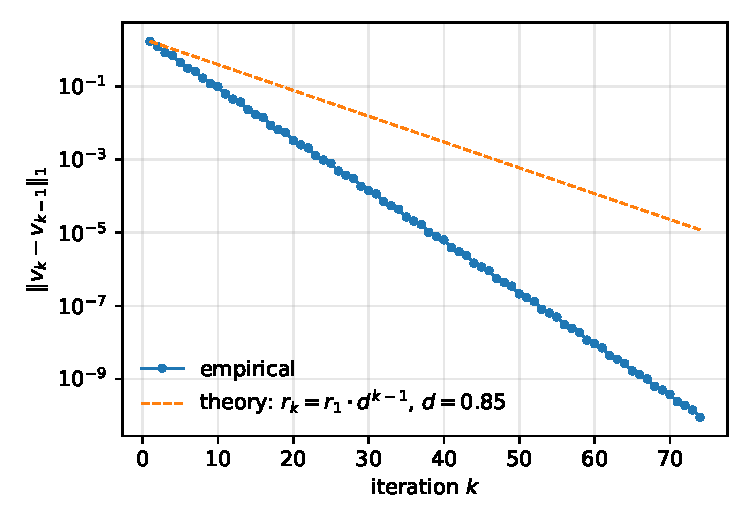
\includegraphics[width=\linewidth]{fig1_convergence.pdf}
  \caption{Convergence of power iteration on the \emph{Attention
  Is All You Need} ego-network ($N = 2{,}504$, $d = 0.85$). The
  residual $\|\mathbf{v}_k - \mathbf{v}_{k-1}\|_1$ shrinks by a
  factor of $\approx 0.729$ per step, faster than the loose bound
  $d = 0.85$ (dashed). Computing $|\lambda_2(P)| = 0.851$
  directly gives the spectral-gap prediction $d \cdot
  |\lambda_2(P)| \approx 0.723$, which matches the observed rate
  within $1\%$.}
  \label{fig:convergence}
\end{figure}

\section{Method B: Damping Sensitivity}
\label{sec:method-b}

Section~\ref{sec:method-a} fixed $d = 0.85$ throughout. The
question now is whether that choice matters: does the ranking
shift much if we slide $d$ across the range the literature
considers reasonable? The damping factor carries two meanings
simultaneously. As a Markov chain parameter, $d$ is the
probability that the walker continues along the graph rather
than teleporting back to the seed. As a linear-algebra
parameter, $d$ is the \emph{contraction factor}. The recursion
shrinks the gap between successive iterates by roughly $d$
each step, which is what makes them converge. These two roles
connect through the teleport itself. Every time the walker
teleports back to $\mathbf{e}_s$, the non-invariant components
of the current iterate shrink by a factor of $d$. A smaller
$d$ teleports more often, converges faster, and biases scores
toward the seed; a larger $d$ explores more of the graph but
converges more slowly.

We used $d = 0.85$ in Section~\ref{sec:method-a} because it is
the value Brin and Page originally chose~\cite{brin1998anatomy}
and the value the PageRank literature has retained ever since.
The choice is conventional rather than derived. A sensible
ranking method should not depend strongly on the exact choice
of its parameters, so we quantify how much the ranking changes
as we vary $d$ across the range $[0.50, 0.99]$.

We compute the Personalized PageRank vector $\mathbf{v}_d$ at
each $d \in \{0.50, 0.60, 0.70, 0.80, 0.85, 0.90, 0.95, 0.99\}$
and record the pairwise Pearson correlation
\begin{equation}
  r(\mathbf{v}_{d_1}, \mathbf{v}_{d_2}) =
  \frac{\operatorname{Cov}(\mathbf{v}_{d_1}, \mathbf{v}_{d_2})}
       {\sigma_{d_1}\, \sigma_{d_2}},
\end{equation}
treating each paper as an observation. This is the correlation
coefficient studied in the covariance-and-correlation chapter of
the course~\cite{nicholson2018linear}. A value close to $1$
indicates that the two score vectors agree up to a linear
transformation, a sufficient condition for them to induce the
same ranking.

\begin{figure}[t]
  \centering
  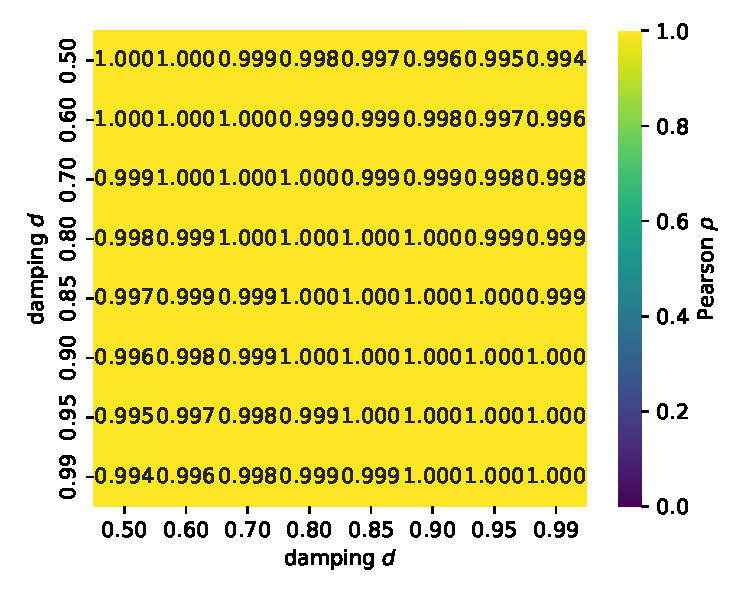
\includegraphics[width=\linewidth]{fig2_damping.pdf}
  \caption{Pairwise Pearson correlation of PPR score vectors
  across damping values on the \emph{Attention Is All You Need}
  ego-network. Every off-diagonal entry exceeds $0.994$; within
  the literature-recommended band $d \in [0.70, 0.95]$, every
  pair exceeds $0.998$.}
  \label{fig:damping}
\end{figure}

Figure~\ref{fig:damping} shows what we get. The lowest
off-diagonal correlation across the entire sweep is
$r(\mathbf{v}_{0.50}, \mathbf{v}_{0.99}) = 0.994$; within the
literature-recommended band $d \in [0.70, 0.95]$, every pair
exceeds $0.998$. For practical purposes the ranking does not
depend on $d$ on this graph at all. Any reasonable choice of damping
produces the same reading list.

Two things drive this stability, and they reinforce each
other. First, the top of the ranking sits well clear of the
rest in absolute score. The seed itself
accounts for $\approx 0.389$ of the total score and the
second-ranked paper for only $\approx 0.024$, so small relative
perturbations cannot reorder the top ranks. Second, $d$ enters $\mathbf{v}$ only through how strongly each
eigenvector of $P$ contributes, not through the eigenvectors
themselves. The dominant structure of $\mathbf{v}$ is set by the
leading eigenvectors of $P$ regardless of damping.

This is a claim about ranks, not absolute scores. Pearson
correlation measures whether two vectors agree up to a linear
transformation, which captures the \emph{ordering} of the
entries but is insensitive to small shifts in the score values
themselves. The distinction matters here: as $d \to 1$, the
smallest
eigenvalue of $I - dP$ is $1 - d$ (corresponding to $\lambda_1
= 1$ of $P$), which approaches zero. Inverting $I - dP$ then
amplifies perturbations by roughly $1/(1-d)$, so small
numerical changes to the graph or the right-hand side can
produce large changes in the score values $\mathbf{v}$. A
linear system with this property is called
\emph{ill-conditioned}~\cite{langville2004deeper}. The scores
wobble; the ranks do not.

\section{Discussion}
\label{sec:discussion}

With convergence and damping stability established, we now ask
whether PPR's ranking actually differs from the simplest
alternative.

\begin{table}[t]
  \centering
  \caption{Top-$20$ papers in the \emph{Attention Is All You
  Need} ego-network ranked by Personalized PageRank versus by
  raw citation count (in-degree). Stars mark papers unique to
  each list. The seed sits at the top of the PPR ranking but
  does not appear in the citation-count top-$20$ at all.}
  \label{tab:rankings}
  \small
  \begin{tabular}{@{}rll@{}}
    \toprule
    Rank & PPR ranking & Citation-count ranking \\
    \midrule
    1  & Vaswani 2017 (seed)$^\star$ & Hochreiter 1997 \\
    2  & Huang 2009                  & Bahdanau 2014 \\
    3  & Kaiser 2016$^\star$         & Sutskever 2014 \\
    4  & Hochreiter 1997             & Cho 2014 \\
    5  & Sutskever 2014              & Graves 2013 \\
    6  & Bahdanau 2014               & Kingma 2014 \\
    7  & Cho 2014                    & He 2015 \\
    8  & Graves 2013                 & Luong 2015 \\
    9  & He 2015                     & Wu 2016 \\
    10 & Kingma 2014                 & Marcus 1993 \\
    11 & Marcus 1993                 & Zhou 2016 \\
    12 & Luong 2015                  & Hochreiter 2001 \\
    13 & McClosky 2006               & Vinyals 2014 \\
    14 & Wu 2016                     & Sennrich 2015 \\
    15 & Petrov 2006                 & Sukhbaatar 2015$^\star$ \\
    16 & Vinyals 2014                & McClosky 2006 \\
    17 & Hochreiter 2001             & Józefowicz 2016 \\
    18 & Zhou 2016                   & Huang 2009 \\
    19 & Józefowicz 2016             & Ba 2016$^\star$ \\
    20 & Sennrich 2015               & Petrov 2006 \\
    \bottomrule
  \end{tabular}
\end{table}

The simplest alternative we can compare against is to rank
papers by raw citation count, that is, by the \emph{in-degree}
of each node in the scraped graph (the number of other papers
in our sample that cite it). Table~\ref{tab:rankings} shows the two top-$20$ lists side by
side. Within the top-$10$ they overlap on $7$ of $10$ papers;
across the full top-$20$, on $18$ of $20$. Where they diverge is
informative.

The most striking difference is at the very top. PPR ranks the
seed itself, \emph{Attention Is All You Need}, at $\#1$, while
the seed does not appear in the citation-count top-$20$ at all.
This difference is the personalization at work. The teleport
vector $\mathbf{e}_s$ sends probability back to the seed at
every step, so the seed accumulates score regardless of how
many scraped papers cite it. In-degree only sees citations
inside our two-hop window, which captures a small fraction of
the seed's total incoming edges.

Within the top-$10$ specifically, the PPR-only entries (Huang
2009, Kaiser 2016) are also direct references of the seed, as
are the citation-count-only entries (Luong 2015, Wu 2016,
Marcus 1993). The difference between the two lists is therefore
not about graph distance: all five papers sit one citation hop
from the seed.

What separates them, then, is how each ranking weights incoming
edges. Across the network as a whole the two scores agree
strongly: the Pearson correlation between PPR and in-degree
(over all $2{,}503$ non-seed papers) comes out at $0.958$, so
the rankings are mostly aligned. The reorderings in
Table~\ref{tab:rankings} are where the structural-versus-popular
distinction surfaces. Citation count weighs every citer equally
and tracks raw in-degree: Luong, Wu, and Marcus carry $59$,
$57$, and $57$ incoming edges in our scrape, above Huang's $53$
and Kaiser's $52$. PPR weighs each incoming edge by the score
of the citer, and the mean PPR score among the citers of Huang
and Kaiser is roughly twice that of the citation-count-only
entries ($\approx 0.015$ versus $\approx 0.008$). Huang and Kaiser are
therefore embedded more deeply in the seed's neighborhood,
while Luong, Wu, and Marcus are cited more often but by
lower-ranked papers.

Three limitations are worth flagging up front. First, the
scrape itself was bounded. We explored outward from the seed, fetching at most
$50$ references and $50$ citations per paper and stopping after
two hops. This
bounds graph size but also truncates papers with dense
citation neighborhoods. Concretely, for the seed
\emph{Attention Is All You Need}, the cap captures all $41$
outgoing references but only $50$ of its $173{,}976$ incoming
citations on Semantic Scholar: full coverage of what the seed
builds on, but a tiny sample of what builds on the seed. Second, the seed choice dominates the
result. The PPR ranking on this graph reflects what is close to
\emph{Attention Is All You Need}, not what is globally important;
running the pipeline with a different seed would scrape a
different ego-network and produce a different ranking. Third,
the Semantic Scholar API~\cite{semanticscholarapi} has real
coverage gaps. In our run,
$56$ of the $89$ papers reachable in one citation hop from the
seed returned null reference data because the publisher had
not released the metadata, and papers outside S2's coverage
entirely cannot be processed at all.

\section{Conclusion}
\label{sec:conclusion}

We modeled academic paper recommendation as Personalized
PageRank on a directed citation ego-network, and we looked at
the resulting system from two angles. Power iteration
converges geometrically at rate $d \cdot |\lambda_2(P)|$, with
the observed contraction ($0.729$) matching the spectral
prediction ($0.723$) within $1\%$. The ranking barely budges under the damping parameter. Pairwise Pearson correlation across
$d \in [0.50, 0.99]$ exceeds $0.994$, so any reasonable choice
of $d$ produces the same reading list. Natural extensions
include deeper scrapes, sparser seeds, and comparison against
topic-model recommenders.

Our code, the canonical scrape, and the figures used in this
paper are available at
\url{https://github.com/hayden1126/PaperRec-submission}.

\balance
\bibliographystyle{IEEEtran}
\bibliography{references}

\end{document}
